\section{Running Example}


\begin{figure}[t]
  \centering
  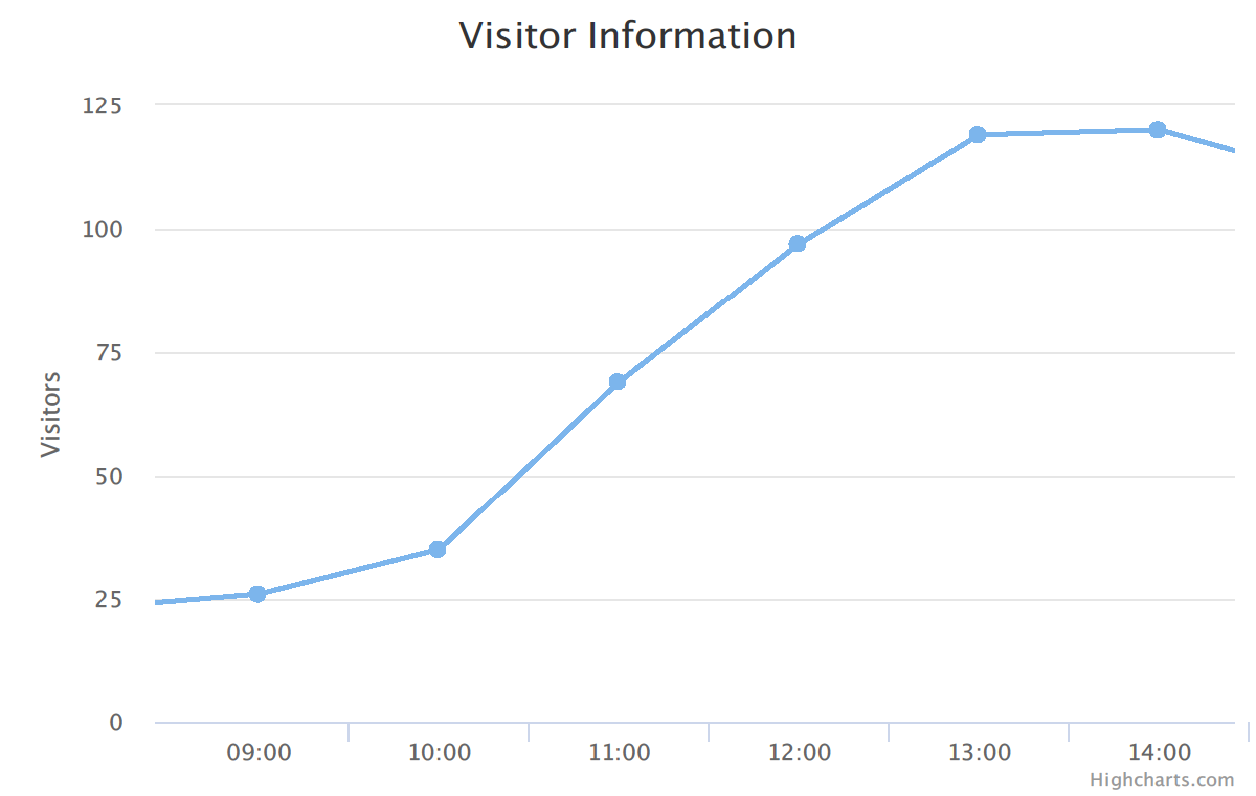
\includegraphics[width=0.8\columnwidth]{figures/first-line.png}
  \caption{Line chart showing visitors per hour}
\label{figure:first-running-example:first-line-chart}
  %\vspace*{\floatsep}% http://tex.stackexchange.com/q/26521/5764
   %\vspace*{0.1cm}
  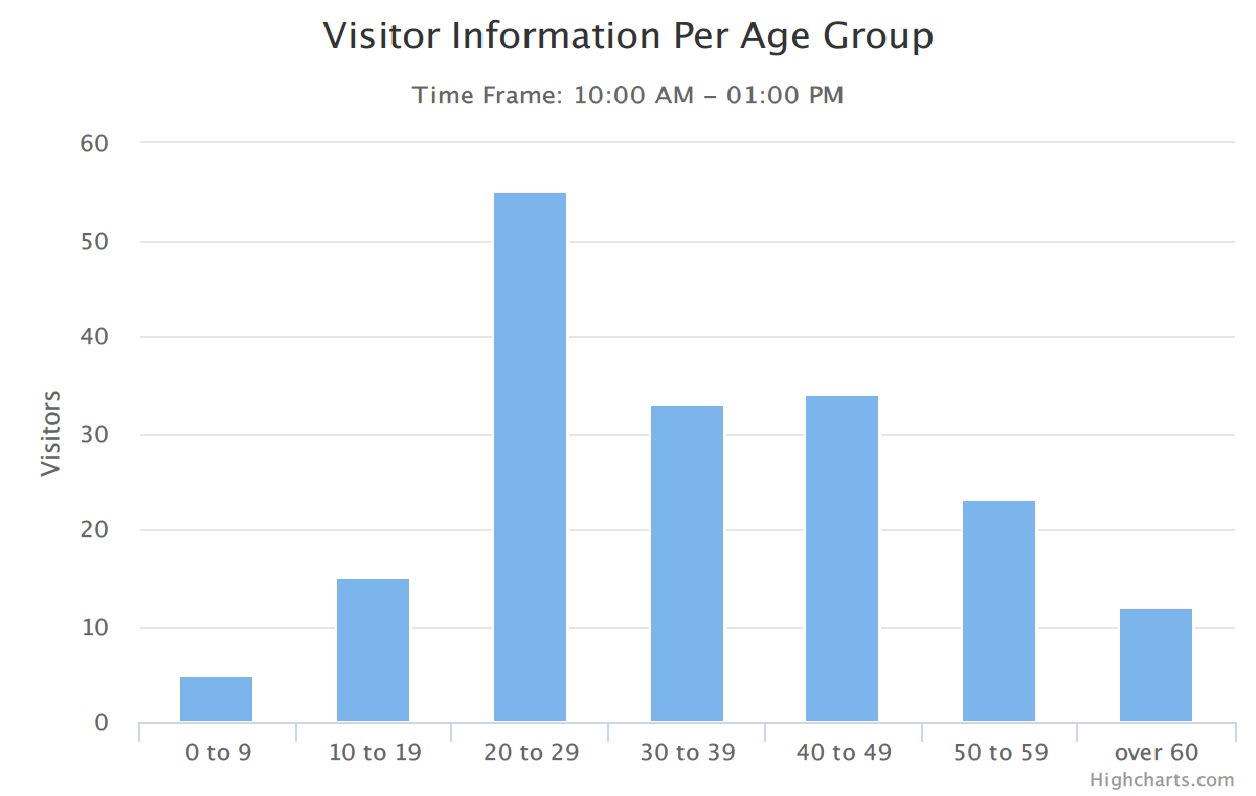
\includegraphics[width=0.8\columnwidth]{figures/first-bar.png}
  \caption{Bar chart showing age groups of visitors}
  \vspace{-15pt}
  \label{figure:first-running-example:first-bar-chart}
  
\end{figure}

\begin{table}
\begin{center}

\begin{tabular}{|c|c|c|c|c|c|}
\hline 
\multicolumn{6}{|c|}{Page Views} \\ 
\hline 
id & vid & url & time & date & revenue \\ 
\hline 
\end{tabular} 

\hfill

\begin{tabular}{|c|c|c|c|c|c|}
\hline 
\multicolumn{6}{|c|}{Visitors} \\ 
\hline 
vid & name & lastname & username & age & gender \\ 
\hline 
\end{tabular} 

\end{center}
\caption{Schema description of database tables.}
\vspace*{-30pt}
\label{tab:schema}

\end{table}


In order to illustrate the issues with existing notebooks and describe the extensions in \projname\, we will use the following example of a potential analysis:

\begin{example}
	
\eat{	
	
Consider a data analyst, working for a news portal website. The analyst wishes to create a notebook that extracts and presents information about the demographics of the website's reader-base during particular hours. More specifically, the analyst wants to construct a chart showing the number of readers that visit the website during the day; then based on this information, she would like to extract the age groups of the visitors, during various hours of that day and present the results to the portal editor. Figure \ref{figure:first-running-example:first-line-chart} shows the graph that displays the number of visitors per hour in a line chart and Figure \ref{figure:first-running-example:first-bar-chart} displays the age groups of the visitors in a bar chart. By doing this, the analyst can convince the portal editor to publish more articles and advertisements that target particular age groups during hours in which they visit the portal the most, thus maximizing the portal's revenue and reader's satisfaction.
}

\eat{
Consider a data analyst, working for a news portal. The analyst wishes to convince the lead editor of the portal that by publishing more articles and advertisements that pertain to particular audiences during specific time-windows of the day, they can maximize the portal's revenue. In order to achieve this, the analyst intends to obtain data that contain the number of readers that visit the website during the day; then for various time-windows she would like to obtain and plot the demographics of the portal's visitors (for instance, the visitors' age groups) during these hours and lastly compute and plot the portal's actual and the predicted revenue. 
}

Consider a data analyst, working for a news portal. The analyst wishes to convince the lead editor of the portal that by publishing more articles and advertisements that pertain to particular audiences during specific time-windows of the day, they can maximize the portal's revenue. In order to achieve this, the analyst intends to obtain and plot the number of readers that visit the website during the day; then for various time-windows she would like to obtain information about the readers' demographics (for instance, the visitors' age groups) and plot the result. Lastly, she would like to compute the portal's actual and predicted revenue (using a linear regression model) and plot the the results, side-by-side, thus illustrating whether there is room for improving revenue. 
\end{example}

Note that, in this example, we can identify two types of users, the code-literate data scientist and the non-technical editor of the portal.

\eat{
\begin{figure}[ht]
  \centering
  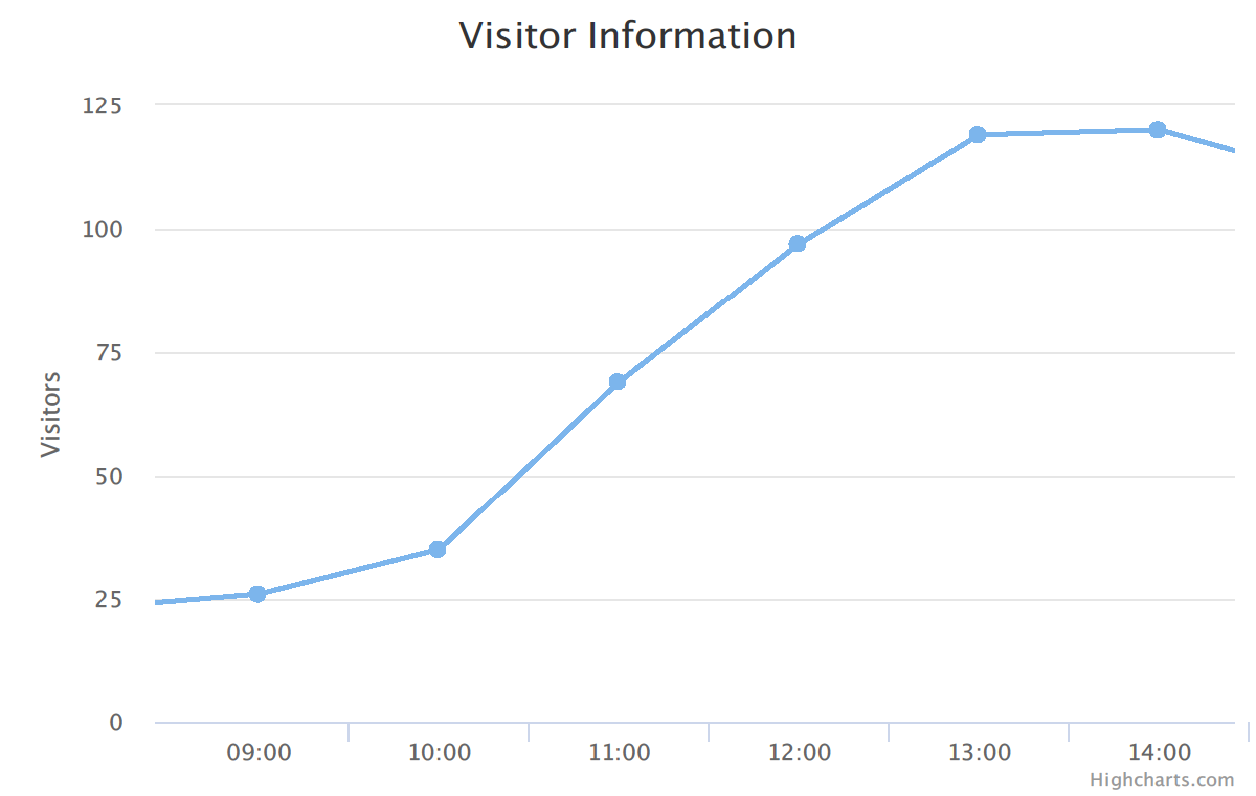
\includegraphics[width=0.8\columnwidth]{figures/first-line.png}
  \caption{Line chart showing visitors per hour}
\label{figure:first-running-example:first-line-chart}
  %\vspace*{\floatsep}% http://tex.stackexchange.com/q/26521/5764
   %\vspace*{0.1cm}
  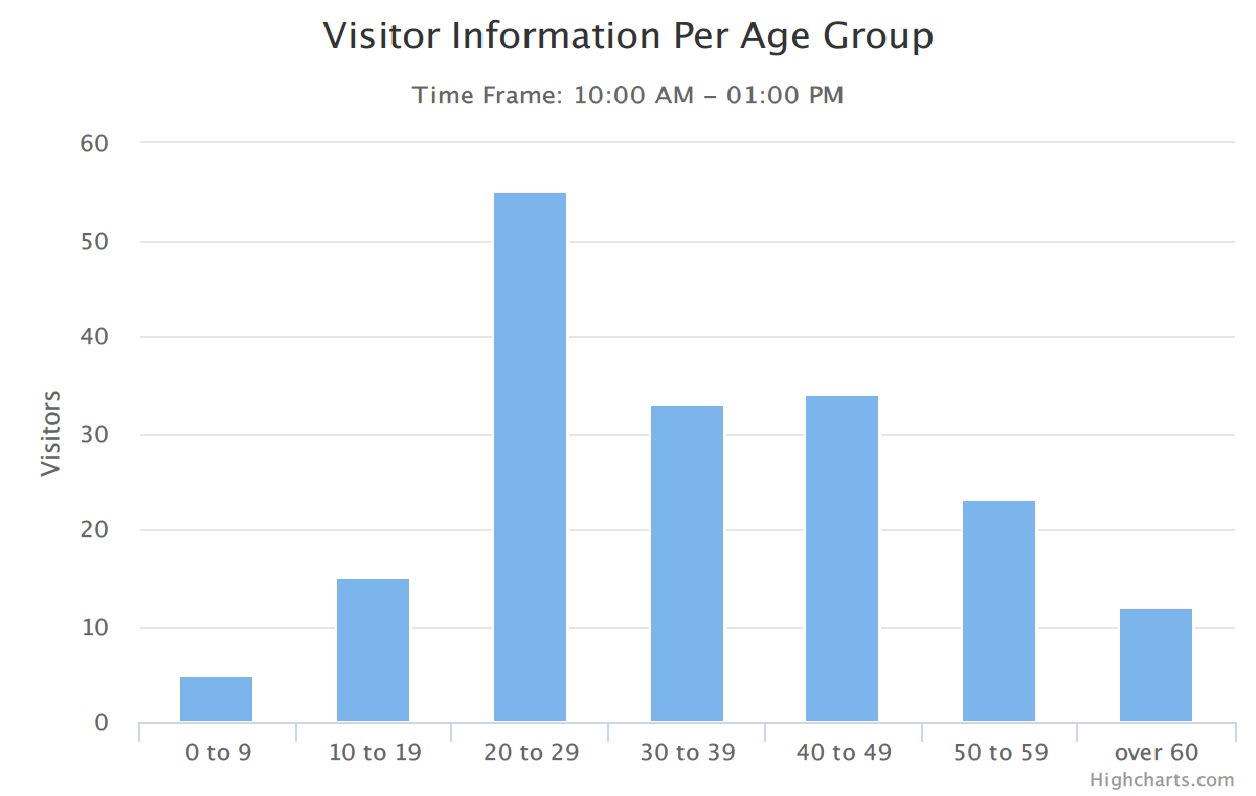
\includegraphics[width=0.8\columnwidth]{figures/first-bar.png}
  \caption{Bar chart showing age groups of visitors}
  \label{figure:first-running-example:first-bar-chart}
\end{figure}
}



\costas{Should section 2 be changed in any way?}



